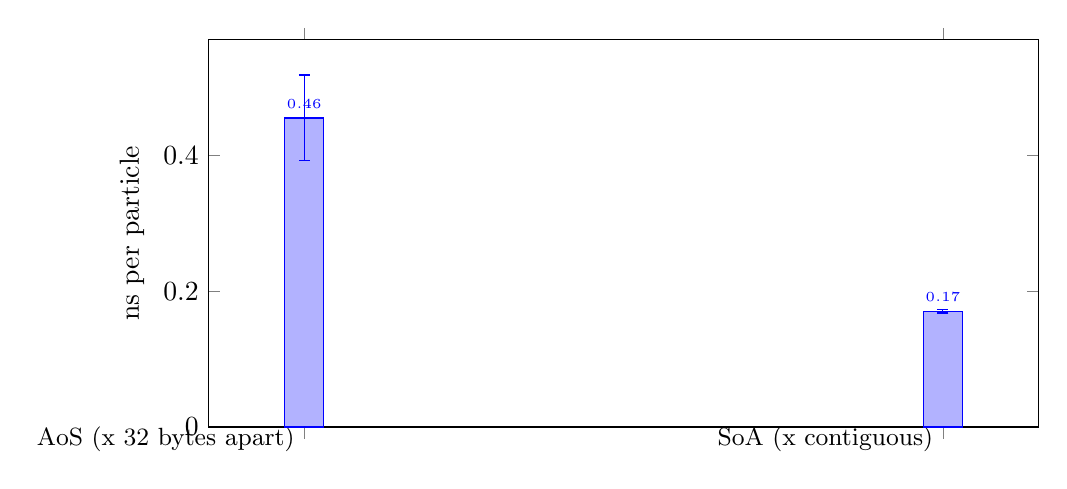
\begin{tikzpicture}
\begin{axis}[ybar, width=\textwidth, height=6.5cm, bar width=14pt, ymin=0, symbolic x coords={AoS (x 32 bytes apart),SoA (x contiguous)}, xtick=data, x tick label style={rotate=0, anchor=east, font=\small}, ylabel={ns per particle}, enlarge x limits=0.15, legend style={font=\small, at={(0.98,0.98)}, anchor=north east}, nodes near coords, nodes near coords style={font=\tiny}, every node near coord/.append style={/pgf/number format/.cd, fixed, precision=2}]
\addplot+[error bars/.cd, y dir=both, y explicit] coordinates {(AoS (x 32 bytes apart),0.4552) +- (0,0.0633) (SoA (x contiguous),0.1704) +- (0,0.0024)};
\end{axis}
\end{tikzpicture}